\documentclass[a4paper,fleqn]{cas-sc}

\usepackage[numbers,sort&compress]{natbib}
\usepackage{longtable}
\usepackage{textcomp}
\graphicspath{{figures/}}

\begin{document}
\let\WriteBookmarks\relax
\def\floatpagepagefraction{1}
\def\textpagefraction{.001}

\shorttitle{Combustion-Informed Smoke Constituent Prediction}
\shortauthors{J. Guo et~al.}

\title [mode = title]{Combustion-Informed Generation And Retention (CIGAR): A Physics-Based Model for Interpretable Prediction of Cigarette Mainstream Smoke Constituents}

\author[1]{Jizhao Guo}
\author[2]{Yihang Zhu}
\author[2]{Fan Wu}
\author[3]{Haifeng Li}
\author[1]{Yipeng Wang}
\author[1]{Peijian Sun}
\author[1]{Bin Peng}
\author[1]{Cong Nie}
\author[1]{Xuehui Sun}
\cormark[1]
\ead{xuehui\_sun1234@aliyun.com}
\author[2]{Qiang Zhang}
\cormark[2]
\ead{qiang.zhang.cs@zju.edu.cn}

\affiliation[1]{organization={Zhengzhou Tobacco Research Institute of CNTC},
                postcode={450001},
                country={China}}

\affiliation[2]{organization={Zhejiang University},
                postcode={314400},
                country={China}}

\affiliation[3]{organization={China Tobacco Zhejiang Industrial Co., Ltd.},
                postcode={310008},
                country={China}}

\cortext[cor1]{Corresponding author.}
\cortext[cor2]{Corresponding author.}

\begin{abstract}
Combustible cigarettes remain the dominant form of tobacco use worldwide and a leading cause of preventable death, prompting efforts to monitor and reduce harmful constituents of mainstream smoke. Predicting these constituents from cigarette design could accelerate regulation and harm assessment, yet existing machine-learning approaches treat cigarettes as black boxes, returning scalar yields without the combustion process that produced them. We developed Combustion-Informed Generation And Retention (CIGAR), an artificial intelligence (AI) contribution that combines a physics-informed hybrid model with a tabular prior-data fitted network (TabPFN)-based formulation factor for the engineering application of cigarette combustion, aerosol filtration, and mainstream-smoke constituent prediction. CIGAR couples a mechanistic simulation of puff-by-puff combustion and filtration, driven by physical design, with a learned formulation-specific generation factor predicted from tobacco chemical composition. Rather than emitting only a scalar yield, CIGAR produces per-puff trajectories of generation at the combustion cone and retention through the tobacco rod and filter sections, with mainstream yield as the endpoint. Under 5-fold cross-validation on a separate formulation-level dataset, CIGAR matches or outperforms extreme gradient boosting (XGBoost) and TabPFN on most constituents, achieving the best mean absolute error on seven of nine and best $R^2$ on six of nine. Because every trajectory step is a physical state rather than a learned latent, the simulation is interpretable by construction and open to inspection at every puff and segment. CIGAR therefore offers regulators and harm-reduction researchers a transparent tool for anticipating how design changes reshape mainstream-smoke toxicants.
\end{abstract}

\begin{highlights}
\item CIGAR couples puff-by-puff combustion simulation with a tobacco formulation-factor predictor.
\item The model predicts mainstream-smoke constituents while exposing generation and retention trajectories.
\item Five-fold cross-validation shows competitive accuracy against XGBoost and TabPFN baselines.
\end{highlights}

\begin{keywords}
Cigarette mainstream smoke \sep Harmful and potentially harmful constituents \sep Physics-informed modeling \sep Mechanistic simulation \sep TabPFN \sep Interpretable machine learning
\end{keywords}

\maketitle

% ==================================================
% MAIN TEXT
% ==================================================

\section{Introduction}

Tobacco use remains one of the largest preventable causes of death and disability worldwide. The World Health Organization (WHO) attributes more than seven million deaths each year to tobacco, including an estimated 1.6 million non-smokers exposed to second-hand smoke \cite{who2025tobacco}, and the Global Burden of Disease Study 2019 ranks smoking among the foremost global risk factors, responsible for an estimated 7.69 million deaths and 200 million disability-adjusted life-years in that year alone \cite{gbd2019tobacco}. This burden falls disproportionately on low- and middle-income countries, where more than 80\% of the world's 1.3 billion tobacco users live \cite{who2025tobacco}, and combustible cigarettes---whose harm arises overwhelmingly from the chemistry of burning rather than from nicotine itself---remain the dominant form of consumption. The scale of this toll has made tobacco control a sustained international priority, formalized in the WHO Framework Convention on Tobacco Control (WHO FCTC), the first treaty negotiated under the auspices of the WHO and now binding on more than 180 Parties \cite{who2003fctc}.

Central to these regulatory efforts is the systematic identification, quantification, and monitoring of Harmful and Potentially Harmful Constituents (HPHCs) in mainstream cigarette emissions. During combustion, a cigarette acts as a highly complex micro-chemical reactor, generating an aerosolized mixture that contains thousands of chemical constituents, hundreds of which are toxic, including well-documented toxicants such as carbon monoxide (CO), tar, nicotine, and various volatile carcinogens \cite{BAKER2006373, ijerph8020613, Hecht2003TobaccoCarcinogens}. Because the released amount of each constituent ultimately governs exposure and risk, accurately quantifying these emissions is paramount for both public-health protection and the advancement of comprehensive tobacco harm-reduction science \cite{Burns2008WHO, HAMMOND2006781, MURPHY2017342}.

While the chemical composition of the tobacco filler supplies the precursor material, the physical design of a cigarette strongly modulates combustion thermodynamics, fluid dynamics, and the resulting yield of harmful gases \cite{BAKER2006373, OConnor2008CigaretteDesign, PMID27222918}. To ensure that emission evaluations are reliable, reproducible, and comparable across markets, regulatory bodies and research institutions worldwide rely on standardized testing protocols built on a common set of measurable physical properties. Geometric specifications (e.g., length and circumference), flow-resistance characteristics (e.g., draw resistance), ventilation distribution, and standardized puffing behavior are widely recognized as the fundamental variables governing combustion dynamics. Leveraging these physical descriptors therefore provides a standardized, internationally communicable basis for analyzing and predicting toxicant yields, largely independent of regional market variation.

Traditionally, determining the amounts of individual smoke constituents requires exhaustive and time-consuming physical experiments. To accelerate safety evaluation and reduce this experimental overhead, recent studies have explored machine learning (ML) as a promising alternative, learning predictive mappings from cigarette properties to mainstream-smoke constituents \cite{yang2022demislim, he2023multifactor, wan2026homogeneity, Zhu2025transformer, Hannel2019AnAF}.

Despite these early advances, prior studies share several limitations that hinder real-world deployment. First, most prior work targets a narrow set of conventional constituents such as CO and tar, neglecting other important toxicants such as hydrogen cyanide (HCN) and phenol. Second, many efforts rely on relatively simple methods such as linear regression, which, although interpretable, cannot match the predictive accuracy of more expressive machine-learning models. Third, many models are developed on single-source datasets, leaving their generalizability across formulations and specifications unverified. Finally, and most fundamentally, prior models treat the cigarette as a black box, returning a single scalar yield with no account of the combustion and filtration process that produced it; this opacity offers regulators little process-level insight into how a given design choice reshapes the emitted toxicant profile.

More broadly, recent work on interpretable and physics-informed machine learning (PIML) has sought to reduce the trade-off between predictive accuracy and transparency. General-purpose interpretability toolboxes, such as PiML and MoDeVa, improve transparency by using interpretable model classes or post-hoc diagnostics for black-box models \cite{Rudin2019InterpretableModels, sudjianto2023piml, modeva_explain_docs}, but they still explain a scalar input--output mapping rather than the latent physical process that produces the output \cite{pmlr-v108-janzing20a, Molnar2022}. Another prominent class of PIML methods is physics-informed neural networks (PINNs), which train neural networks not only to fit observational data but also to minimize residuals of governing differential equations, often together with initial and boundary condition terms \cite{RAISSI2019686, Karniadakis2021PhysicsInformedML, Cuomo2022PINN}. For cigarette mainstream-smoke prediction, however, a compact semi-empirical model is more practical than solving or constraining a full PDE model across the burning cigarette at population-data scale. Such a model can encode puff-level generation and segment-level penetration directly while fitting its parameters end-to-end against measured mainstream yields.

To address these critical gaps, we introduce CIGAR (Combustion-Informed Generation And Retention), a physics-informed model that couples a mechanistic simulation of a cigarette's puff-by-puff combustion and filtration, driven by its physical design, with a learned formulation-specific generation factor predicted from tobacco chemical composition through a dedicated TabPFN stage. Rather than predicting a single scalar yield, CIGAR generates the full per-puff trajectory of generation at the combustion cone and the retention through rod and filter; the measured mainstream yield is its endpoint, not its sole output. We show that CIGAR attains predictive accuracy comparable to strong ML models while producing this simulated trajectory as a native by-product of inference --- a process-level account of how cigarette design propagates to mainstream emissions that black-box tabular models cannot provide. Interpretability follows as a consequence: because each step of the trajectory corresponds to a physical state rather than a learned latent, the simulation can be inspected against domain knowledge at every puff and every segment.

\section{Results}

\subsection{Characteristics of the Dataset and Features}

The data used in this study were drawn from 16 independent archived projects of cigarette combustion tests conducted by the Tobacco Research Institute under standardized laboratory protocols and standard testing methods \cite{gb19609,gb23356,yc253,gb23228,yc377,gb21130,yc255,yc254}. Fifteen of these projects, corresponding to 15 distinct tobacco formulations, were integrated into the primary physical-property dataset, which contains 885 cigarette samples used for model development. The remaining project forms an additional formula-level dataset in which each sample represents one tobacco formulation, yielding 262 samples in total; it carries the same cigarette physical descriptors as the primary dataset and additionally records tobacco-composition features for each formula (Table~\ref{tab:dataset_summary}).

\begin{table}[pos=h]
    \centering
    \caption{Summary of the two datasets used in this study.}
    \label{tab:dataset_summary}
    \begin{tabular}{p{0.24\textwidth} p{0.33\textwidth} p{0.33\textwidth}}
        \toprule
        Dataset & Source and scope & Role in the analysis \\
        \midrule
        Dataset 1: physical-property dataset & 15 projects with distinct tobacco formulae; cigarette-level measurements collected under standard methods; up to 885 samples & Main dataset for model training \\
        Dataset 2: formula-level tobacco-composition dataset & One project with 262 formula-level samples; each sample represents one tobacco formula and includes cigarette physical descriptors plus tobacco-composition measurements & Additional feature-rich dataset for chemical factor prediction and testing \\
        \bottomrule
    \end{tabular}
\end{table}

To distinguish the same compound in the predictor and response spaces, we refer to NNK measured in unburned tobacco as tobacco NNK content ($\mathrm{NNK}_{\mathrm{tob}}$), an input feature, and NNK released in mainstream smoke as mainstream-smoke NNK yield ($\mathrm{NNK}_{\mathrm{smoke}}$), an output target.

Because the analytical targets varied across the original experiments in the primary physical-property dataset, the number of valid observations differs by smoke constituent. CO, tar, and nicotine, which are internationally recognized smoke indicators~\cite{Burns2008WHO}, were measured across all samples, whereas the remaining constituents were available for smaller subsets of 471--513 samples (Table \ref{tab:target_sample_counts}). The target counts reported here therefore refer to the primary dataset used in the main predictive experiments.

\begin{table}[pos=h]
    \centering
    \caption{Number of valid samples for each target in Dataset 1.}
    \label{tab:target_sample_counts}
    \begin{tabular}{lr}
        \toprule
        Target & n\_samples \\
        \midrule
        CO (mg) & 885 \\
        HCN (\textmu g) & 495 \\
        Phenol (\textmu g) & 495 \\
        Crotonaldehyde (\textmu g) & 513 \\
        NH$_3$ (\textmu g) & 471 \\
        BaP (\textmu g) & 495 \\
        Mainstream-smoke NNK yield ($\mathrm{NNK}_{\mathrm{smoke}}$; \textmu g) & 495 \\
        Tar (mg) & 885 \\
        Nicotine (mg) & 885 \\
        \bottomrule
    \end{tabular}
\end{table}

Feature selection and engineering were guided by domain expertise rather than purely data-driven screening. The cigarette-level variables capture puff-resolved burning geometry and air-intake behavior, together with structural and flow-resistance descriptors of the cigarette. Specifically, the raw physical measurements include tobacco filler length per puff; combustion-cone, cigarette-paper, and ventilation-hole air intake per puff; cigarette circumference; filter length before and after the ventilation holes; tobacco-segment standard closed draw resistance; filter-rod standard draw resistance; and number of puffs. These measurements describe mechanistic aspects of cigarette design and smoking dynamics that plausibly influence combustion, dilution, and constituent transfer.

The formula-level dataset adds tobacco-composition variables that are not available in the 15-project physical-property dataset. These variables include tobacco weight and tobacco-segment draw resistance; proximate chemical indices, such as reducing sugar, total sugar, total alkaloids, total nitrogen, and starch; polyphenols and related compounds, including neochlorogenic acid, chlorogenic acid, 4-O-caffeoylquinic acid, scopoletin, and rutin; organic acids, including oxalic, malonic, succinic, malic, and citric acids; fatty acids, including palmitic, linoleic, oleic plus linolenic, and stearic acids; amino acids, including Asp, Thr, Ser, Asn, Glu, Ala, Leu, Tyr, Phe, His, and Pro; inorganic ions and elements, including chloride, sulfate, phosphate, Mg, K, and Ca; and tobacco NNK content ($\mathrm{NNK}_{\mathrm{tob}}$). The resulting feature structure comprises a shared cigarette-design layer and an additional tobacco-formula layer (Table \ref{tab:feature_dimensions}).

\begin{table}[pos=h]
    \centering
    \caption{Feature families represented in the two datasets.}
    \label{tab:feature_dimensions}
    \begin{tabular}{p{0.30\textwidth} p{0.62\textwidth}}
        \toprule
        Feature family & Variables \\
        \midrule
        Puff-resolved cigarette geometry & Tobacco filler length per puff \\
        Puff-resolved air-intake distribution & Combustion-cone, cigarette-paper, and ventilation-hole air intake per puff \\
        Cigarette construction and flow resistance & Cigarette circumference, filter length before/after ventilation holes, tobacco-segment standard closed draw resistance, filter-rod standard draw resistance, number of puffs \\
        Tobacco-formula composition & Tobacco weight, tobacco-segment draw resistance, sugars, alkaloids, nitrogen, starch, polyphenols, organic acids, fatty acids, amino acids, inorganic ions/elements, and tobacco NNK content ($\mathrm{NNK}_{\mathrm{tob}}$) \\
        \bottomrule
    \end{tabular}
\end{table}

Figure~\ref{fig:flow} summarizes the overall CIGAR pipeline.

\begin{figure}[pos=h]
    \centering
    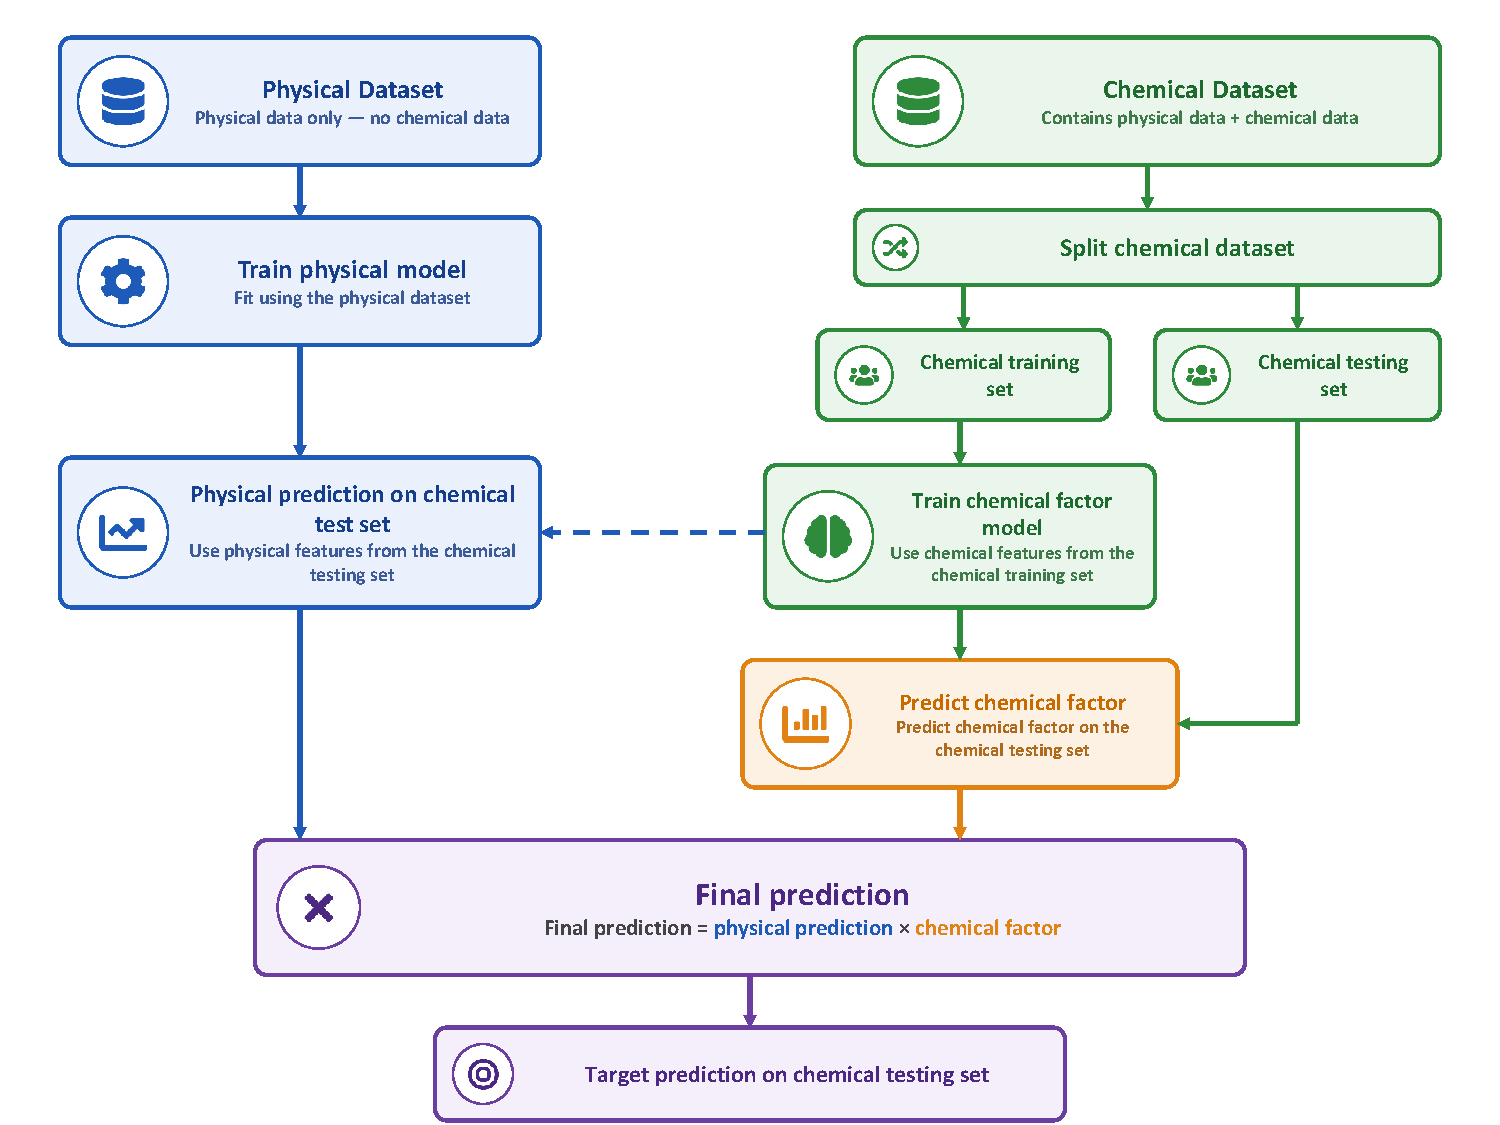
\includegraphics[width=0.9\textwidth]
    {Physical-Chemical Prediction Flowchart.pdf}
    \caption{Overview of the CIGAR two-stage modeling and evaluation
    pipeline. The mechanistic release model (``physical model'') is
    trained on the physical-property dataset (Dataset~1) and then
    applied to the physical descriptors of each held-out formulation in
    the formula-level chemical dataset (Dataset~2) to produce a
    neutral-formulation baseline prediction. In parallel, Dataset~2 is
    split into training and test partitions; on the training partition a
    TabPFN regressor (``chemical-factor model'') learns to predict the
    formulation-specific generation factor $k_G$ from tobacco chemical
    composition, and then predicts it for the test partition. The final
    mainstream-yield prediction for each test sample is the product of
    the mechanistic baseline and the predicted formulation factor.}
    \label{fig:flow}
\end{figure}

\subsection{CIGAR achieves competitive predictive accuracy}

CIGAR was designed primarily for interpretability, but a mechanistic model is
only useful if it predicts well enough to be trusted. We therefore first
benchmarked CIGAR against two strong tabular baselines, XGBoost and TabPFN
(Table~\ref{tab:model_experiments}),
under 5-fold cross-validation on Dataset~2 (\texttt{sklearn.KFold},
\texttt{shuffle=True}, \texttt{random\_state=42}); for each fold the
20\% test partition served as the held-out evaluation set and the
remaining 80\% supplied chemical-stage training data. Within each fold
the three models drew on the same per-fold data pool---Dataset~1
together with the fold's 80\% partition of Dataset~2---but partitioned
and consumed it as each model's architecture requires: the baselines
fit jointly on all of Dataset~1 and Part~A$_k$, whereas CIGAR fits its
mechanistic stage on the Dataset~1 train split (a fixed 20\% validation
split held out for early stopping) and its chemical stage on Part~A$_k$,
under the protocol described in STAR Methods. Classic distance-based models such as Support Vector
Machines were not considered, as they typically underperform tree-based
and foundation models on tabular data~\cite{grinsztajn2022tree,SHMUEL2025benchmark}.

\begin{table}[pos=h]
    \centering
    \caption{Models evaluated in this study.}
    \label{tab:model_experiments}
    \begin{tabular}{lll}
        \toprule
        Model & Type & Role \\
        \midrule
        XGBoost & Gradient-boosted tree ensemble & Data-driven baseline \\
        TabPFN  & Tabular foundation model & Data-driven baseline \\
        CIGAR   & Physics-informed two-stage model & Proposed model \\
        \bottomrule
    \end{tabular}
\end{table}

Table~\ref{tab:model_comparison} reports MAE, MSE, MAPE, and $R^2$ for
each constituent as mean~$\pm$~standard deviation across the five test
folds. CIGAR attains the best MAE on seven of the nine constituents (HCN,
Phenol, NH$_3$, BaP, $\mathrm{NNK}_{\mathrm{smoke}}$, Tar, Nicotine) and the best $R^2$ on six (HCN,
Phenol, NH$_3$, BaP, $\mathrm{NNK}_{\mathrm{smoke}}$, Nicotine); on Tar it leads on MAE, MSE, and
MAPE while trailing XGBoost on $R^2$ by 0.006. Two constituents are
exceptions: XGBoost is the strongest model on CO, leading on all four
metrics, and TabPFN is the strongest on Crotonaldehyde, again leading on
all four. On the remaining six targets---HCN, Phenol, NH$_3$, BaP,
$\mathrm{NNK}_{\mathrm{smoke}}$, and Nicotine---CIGAR leads on all four metrics.

{\footnotesize\setlength{\tabcolsep}{4pt}
\begin{longtable}{>{\raggedright\arraybackslash}p{0.10\textwidth} >{\raggedright\arraybackslash}p{0.09\textwidth} >{\centering\arraybackslash}p{0.17\textwidth} >{\centering\arraybackslash}p{0.18\textwidth} >{\centering\arraybackslash}p{0.16\textwidth} >{\centering\arraybackslash}p{0.16\textwidth}}
    \caption{Predictive performance of XGBoost, TabPFN, and CIGAR
    under 5-fold cross-validation on Dataset~2
    (\texttt{sklearn.KFold}, \texttt{shuffle=True},
    \texttt{random\_state=42}). Each entry reports
    mean~$\pm$~standard deviation across the five test folds. For
    each target, the best value per metric is shown in bold. Lower
    is better for MAE, MSE, and MAPE; higher is better for $R^2$.}
    \label{tab:model_comparison} \\

    \toprule
    \textbf{Target} & \textbf{Model} & \textbf{MAE} & \textbf{MSE} & \textbf{MAPE} & \textbf{$R^2$} \\
    \midrule
    \endfirsthead

    \multicolumn{6}{c}%
    {{\bfseries \tablename\ \thetable{} -- continued from previous page}} \\
    \toprule
    \textbf{Target} & \textbf{Model} & \textbf{MAE} & \textbf{MSE} & \textbf{MAPE} & \textbf{$R^2$} \\
    \midrule
    \endhead

    \midrule
    \multicolumn{6}{r}{{Continued on next page...}} \\
    \endfoot

    \bottomrule
    \endlastfoot

    % --- Data Section ---
    \textbf{CO}
    & XGBoost & $\mathbf{0.7323 \pm 0.0371}$ & $\mathbf{0.9398 \pm 0.1131}$ & $\mathbf{0.0521 \pm 0.0028}$ & $\mathbf{0.6104 \pm 0.0699}$ \\
    & TabPFN  & $0.8849 \pm 0.0632$         & $1.3141 \pm 0.2541$         & $0.0614 \pm 0.0036$         & $0.4701 \pm 0.0334$ \\
    & CIGAR   & $0.7725 \pm 0.0568$         & $1.0485 \pm 0.1465$         & $0.0544 \pm 0.0036$         & $0.5667 \pm 0.0838$ \\
    \midrule
    \textbf{HCN}
    & XGBoost & $9.5262 \pm 0.6497$           & $154.4555 \pm 28.5683$          & $0.0938 \pm 0.0022$         & $0.6859 \pm 0.0610$ \\
    & TabPFN  & $10.8636 \pm 0.9053$          & $208.3615 \pm 44.6461$          & $0.1084 \pm 0.0096$         & $0.5782 \pm 0.0819$ \\
    & CIGAR   & $\mathbf{7.6370 \pm 0.5232}$  & $\mathbf{109.1994 \pm 22.0244}$ & $\mathbf{0.0724 \pm 0.0038}$ & $\mathbf{0.7792 \pm 0.0400}$ \\
    \midrule
    \textbf{Phenol}
    & XGBoost & $3.2187 \pm 0.2550$          & $16.6740 \pm 2.3144$          & $0.1169 \pm 0.0071$         & $0.7208 \pm 0.0532$ \\
    & TabPFN  & $3.4339 \pm 0.4586$          & $18.6088 \pm 4.3331$          & $0.1267 \pm 0.0180$         & $0.6908 \pm 0.0730$ \\
    & CIGAR   & $\mathbf{2.8333 \pm 0.1578}$ & $\mathbf{13.1537 \pm 0.5787}$ & $\mathbf{0.1017 \pm 0.0049}$ & $\mathbf{0.7775 \pm 0.0436}$ \\
    \midrule
    \textbf{Crotonaldehyde}
    & XGBoost & $2.1024 \pm 0.2271$          & $7.1291 \pm 1.4675$          & $0.0910 \pm 0.0110$         & $0.3145 \pm 0.0782$ \\
    & TabPFN  & $\mathbf{2.0177 \pm 0.1679}$ & $\mathbf{6.7122 \pm 1.4070}$ & $\mathbf{0.0859 \pm 0.0100}$ & $\mathbf{0.3553 \pm 0.0453}$ \\
    & CIGAR   & $2.0726 \pm 0.1970$          & $7.1718 \pm 1.7436$          & $0.0897 \pm 0.0101$         & $0.3136 \pm 0.1088$ \\
    \midrule
    \textbf{NH$_3$}
    & XGBoost & $1.6168 \pm 0.1684$          & $5.0141 \pm 1.7698$          & $0.1494 \pm 0.0150$         & $0.7004 \pm 0.0543$ \\
    & TabPFN  & $1.7824 \pm 0.1784$          & $5.7216 \pm 1.7804$          & $0.1723 \pm 0.0150$         & $0.6555 \pm 0.0539$ \\
    & CIGAR   & $\mathbf{1.4288 \pm 0.2025}$ & $\mathbf{4.5105 \pm 2.3570}$ & $\mathbf{0.1294 \pm 0.0084}$ & $\mathbf{0.7371 \pm 0.0840}$ \\
    \midrule
    \textbf{BaP}
    & XGBoost & $1.7227 \pm 0.1337$          & $5.1141 \pm 1.1390$          & $0.1002 \pm 0.0093$         & $0.4797 \pm 0.0862$ \\
    & TabPFN  & $2.0285 \pm 0.2877$          & $6.8629 \pm 2.0775$          & $0.1223 \pm 0.0231$         & $0.3069 \pm 0.1675$ \\
    & CIGAR   & $\mathbf{1.6768 \pm 0.2325}$ & $\mathbf{4.9633 \pm 1.3452}$ & $\mathbf{0.0970 \pm 0.0128}$ & $\mathbf{0.4998 \pm 0.0956}$ \\
    \midrule
    \textbf{NNK}
    & XGBoost & $1.3259 \pm 0.1734$          & $6.2001 \pm 2.1517$          & $0.2193 \pm 0.0373$         & $0.6950 \pm 0.0372$ \\
    & TabPFN  & $1.2082 \pm 0.1876$          & $5.7092 \pm 4.7518$          & $0.1964 \pm 0.0238$         & $0.6113 \pm 0.4428$ \\
    & CIGAR   & $\mathbf{1.1253 \pm 0.0743}$ & $\mathbf{4.1246 \pm 1.8255}$ & $\mathbf{0.1878 \pm 0.0197}$ & $\mathbf{0.7447 \pm 0.1934}$ \\
    \midrule
    \textbf{Tar}
    & XGBoost & $0.7281 \pm 0.0734$          & $0.8648 \pm 0.2208$          & $0.0460 \pm 0.0045$         & $\mathbf{0.7712 \pm 0.0236}$ \\
    & TabPFN  & $0.9589 \pm 0.1271$          & $1.5053 \pm 0.3434$          & $0.0596 \pm 0.0075$         & $0.5920 \pm 0.1003$ \\
    & CIGAR   & $\mathbf{0.6988 \pm 0.0304}$ & $\mathbf{0.8632 \pm 0.0668}$ & $\mathbf{0.0434 \pm 0.0020}$ & $0.7650 \pm 0.0269$ \\
    \midrule
    \textbf{Nicotine}
    & XGBoost & $0.1268 \pm 0.0144$          & $0.0297 \pm 0.0073$          & $0.0755 \pm 0.0126$         & $0.8329 \pm 0.0630$ \\
    & TabPFN  & $0.2716 \pm 0.0595$          & $0.1178 \pm 0.0524$          & $0.1449 \pm 0.0243$         & $0.3982 \pm 0.1817$ \\
    & CIGAR   & $\mathbf{0.1127 \pm 0.0084}$ & $\mathbf{0.0249 \pm 0.0078}$ & $\mathbf{0.0669 \pm 0.0046}$ & $\mathbf{0.8603 \pm 0.0547}$ \\
\end{longtable}
}


These results establish that CIGAR's mechanistic structure does not come
at the cost of predictive quality: it matches or outperforms strong
black-box tabular models on the majority of constituents while exposing a
physical mechanism the baselines cannot. The next subsection focuses on
what CIGAR uniquely offers --- a prediction that is mechanistically
inspectable.

\subsection{CIGAR exposes the mechanism behind every prediction}

Unlike the data-driven baselines, every CIGAR prediction decomposes
explicitly into the physical processes formulated in STAR Methods. For
each cigarette and each puff $j$, the model reports the amount $G_{ij}$
generated at the combustion cone, the segment-level air velocities $V$,
the kinetic coefficients $(k_1, k_2, k_3)$, the evolving particle-phase
fraction $a^{\mathrm{out}}$, and the per-segment penetration factors
$\eta^{\mathrm{rod}}_{ij}$, $\eta^{\mathrm{pre}}_{ij}$, and $\eta^{\mathrm{post}}_{ij}$ through the tobacco rod and the two filter
sections, before summing what is released into the mainstream. CIGAR
therefore turns a single scalar yield prediction into a puff-resolved,
segment-resolved report. As a worked example,
Table~\ref{tab:mechanism_breakdown} reports the full mechanism breakdown
produced by CIGAR for sample JH-7, a Dataset~2 cigarette evaluated in one
of the five cross-validation test folds with CO as the target. As the cigarette burns and the tobacco rod
shortens, its penetration factor $\eta^{\mathrm{rod}}$ rises from $0.41$
at puff~1 to $0.83$ at puff~10, while both filter penetration factors
decrease modestly (pre-vent: $0.80\!\to\!0.67$; post-vent:
$0.77\!\to\!0.67$) as the gas-phase fraction reaching the filter
sections grows over the course of the cigarette. The per-puff released
yield consequently rises from $0.87\,\mathrm{mg}$ at puff~1 to
$1.67\,\mathrm{mg}$ at puff~10. A black-box model would report only the
scalar endpoint; CIGAR additionally returns the full trajectory and the
segment-level state that produced it. Figure~\ref{fig:mechanism_trajectory} visualizes the process.

\begin{table}[H]
    \centering
    \caption{Per-puff and per-segment mechanism breakdown predicted by
    CIGAR for sample JH-7, a Dataset~2 cigarette evaluated in one of
    the five cross-validation test folds (target: CO,
    $k_G = 0.8333$, $J = 10$ puffs). Each puff occupies three rows
    for the tobacco rod and the pre- and post-vent filter sections.
    $V$ is the segment air velocity; $k_1$, $k_2$, $k_3$ are the
    kinetic coefficients; $a^{\mathrm{out}}$ is the particle-phase
    fraction leaving the segment; $\eta$ is the segment penetration
    factor; $G_j$ is the puff-level generation at the combustion
    cone; $y_j$ is the per-puff released yield; the rightmost column
    is the cumulative release. All yields are in mg. Fitted physical
    parameters for this constituent were
    $G_1 = -1.53\!\times\!10^{-4}$, $G_2 = 0.1386$,
    $G_3 = 1.0292$, $a_0 = 0.5024$,
    $(m, n, p)_{\mathrm{rod}} = (-0.2674,\, 1.4157,\, 1.6315)$, and
    $(m, n, p)_{\mathrm{fil}} = (-0.2206,\, 1.5589,\, 1.5559)$.
    Some fitted values (e.g.\ $G_2$, $G_3$) fall outside the
    initialization ranges in Table~\ref{tab:init_ranges}, which guided
    initialization only and were not enforced as hard constraints. The
    measured CO yield is $12.70\,\mathrm{mg}$; CIGAR predicts
    $12.28\,\mathrm{mg}$ (absolute error $0.42\,\mathrm{mg}$).}
    \label{tab:mechanism_breakdown}
    \footnotesize
    \setlength{\tabcolsep}{3pt}
    \begin{tabular}{c l c c c c c c c c c}
        \toprule
        Puff & Seg & $V$ & $k_1$ & $k_2$ & $k_3$ & $a^{\mathrm{out}}$ & $\eta$ & $G_j$ & $y_j$ & Cum. \\
        \midrule
        \multirow{3}{*}{1}  & rod  & 31.2867 & 0.4951 & 0.0599 & 0.0521 & 0.9517 & 0.4078 & 3.4698 & 0.8674 & 0.8674 \\
                            & pre  & 37.2795 & 0.7606 & 0.1812 & 0.0417 & 0.9750 & 0.8010 &        &        &        \\
                            & post & 37.2795 & 0.7606 & 0.1812 & 0.0417 & 0.9894 & 0.7654 &        &        &        \\
        \midrule
        \multirow{3}{*}{2}  & rod  & 31.8241 & 0.4905 & 0.0589 & 0.0513 & 0.9357 & 0.4302 & 3.5831 & 0.9331 & 1.8005 \\
                            & pre  & 37.1845 & 0.7612 & 0.1814 & 0.0418 & 0.9665 & 0.7948 &        &        &        \\
                            & post & 37.1845 & 0.7612 & 0.1814 & 0.0418 & 0.9857 & 0.7616 &        &        &        \\
        \midrule
        \multirow{3}{*}{3}  & rod  & 32.3851 & 0.4858 & 0.0580 & 0.0504 & 0.9152 & 0.4554 & 3.6986 & 1.0030 & 2.8035 \\
                            & pre  & 37.1076 & 0.7616 & 0.1815 & 0.0419 & 0.9555 & 0.7869 &        &        &        \\
                            & post & 37.1076 & 0.7616 & 0.1815 & 0.0419 & 0.9809 & 0.7568 &        &        &        \\
        \midrule
        \multirow{3}{*}{4}  & rod  & 32.9668 & 0.4811 & 0.0571 & 0.0495 & 0.8893 & 0.4842 & 3.8156 & 1.0777 & 3.8813 \\
                            & pre  & 37.0474 & 0.7620 & 0.1816 & 0.0420 & 0.9412 & 0.7770 &        &        &        \\
                            & post & 37.0474 & 0.7620 & 0.1816 & 0.0420 & 0.9746 & 0.7507 &        &        &        \\
        \midrule
        \multirow{3}{*}{5}  & rod  & 33.5653 & 0.4763 & 0.0562 & 0.0486 & 0.8573 & 0.5179 & 3.9338 & 1.1577 & 5.0390 \\
                            & pre  & 37.0024 & 0.7622 & 0.1817 & 0.0420 & 0.9230 & 0.7648 &        &        &        \\
                            & post & 37.0024 & 0.7622 & 0.1817 & 0.0420 & 0.9664 & 0.7430 &        &        &        \\
        \midrule
        \multirow{3}{*}{6}  & rod  & 34.1762 & 0.4714 & 0.0554 & 0.0477 & 0.8185 & 0.5580 & 4.0522 & 1.2437 & 6.2826 \\
                            & pre  & 36.9706 & 0.7624 & 0.1818 & 0.0421 & 0.9001 & 0.7501 &        &        &        \\
                            & post & 36.9706 & 0.7624 & 0.1818 & 0.0421 & 0.9558 & 0.7333 &        &        &        \\
        \midrule
        \multirow{3}{*}{7}  & rod  & 34.7940 & 0.4666 & 0.0546 & 0.0469 & 0.7727 & 0.6064 & 4.1701 & 1.3366 & 7.6193 \\
                            & pre  & 36.9501 & 0.7626 & 0.1818 & 0.0421 & 0.8720 & 0.7327 &        &        &        \\
                            & post & 36.9501 & 0.7626 & 0.1818 & 0.0421 & 0.9425 & 0.7214 &        &        &        \\
        \midrule
        \multirow{3}{*}{8}  & rod  & 35.4126 & 0.4619 & 0.0539 & 0.0461 & 0.7200 & 0.6656 & 4.2866 & 1.4379 & 9.0572 \\
                            & pre  & 36.9384 & 0.7626 & 0.1818 & 0.0421 & 0.8379 & 0.7127 &        &        &        \\
                            & post & 36.9384 & 0.7626 & 0.1818 & 0.0421 & 0.9257 & 0.7071 &        &        &        \\
        \midrule
        \multirow{3}{*}{9}  & rod  & 36.0251 & 0.4574 & 0.0532 & 0.0453 & 0.6612 & 0.7389 & 4.4006 & 1.5491 & 10.6063 \\
                            & pre  & 36.9333 & 0.7627 & 0.1818 & 0.0421 & 0.7975 & 0.6904 &        &        &        \\
                            & post & 36.9333 & 0.7627 & 0.1818 & 0.0421 & 0.9049 & 0.6901 &        &        &        \\
        \midrule
        \multirow{3}{*}{10} & rod  & 36.6236 & 0.4529 & 0.0526 & 0.0445 & 0.5974 & 0.8302 & 4.5110 & 1.6727 & 12.2790 \\
                            & pre  & 36.9320 & 0.7627 & 0.1818 & 0.0421 & 0.7507 & 0.6663 &        &        &        \\
                            & post & 36.9320 & 0.7627 & 0.1818 & 0.0421 & 0.8795 & 0.6704 &        &        &        \\
        \bottomrule
    \end{tabular}
\end{table}


\begin{figure}[pos=h]
    \centering
    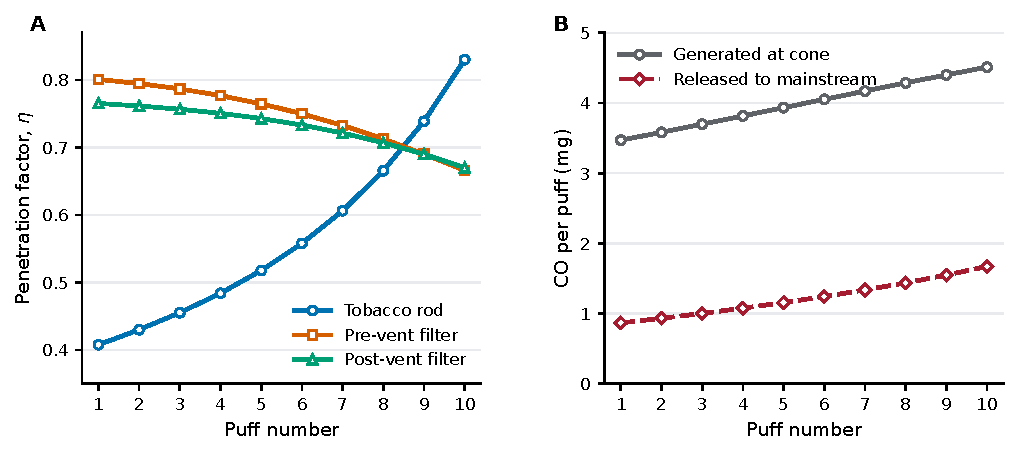
\includegraphics[width=\textwidth]{MechanismTrajectory.pdf}
    \caption{Puff-resolved mechanism trajectories predicted by CIGAR for sample JH-7. (A) Segment penetration factors through the tobacco rod and the pre- and post-vent filter sections across ten puffs. (B) CO generated at the combustion cone and released to mainstream smoke during each puff.}
    \label{fig:mechanism_trajectory}
\end{figure}

Neither XGBoost nor TabPFN can produce this view. Their
predictions are scalar outputs of a black-box function over the input
features, with no internal state that corresponds to per-puff generation,
per-segment retention, or the evolution of the particle-phase fraction.
CIGAR's mechanistic structure makes these quantities a natural by-product
of inference rather than a post-hoc approximation.

% --------------------------------------------------

\section{Discussion}

This study set out to move beyond black-box prediction of toxic mainstream-smoke constituents toward an inspectable, process-level simulation of the combustion that produces them---coupling a cigarette's physical design with its tobacco chemical composition---and to benchmark this approach against strong data-driven models. We summarize our contributions as follows:

(1) We aggregated cigarette samples of different designs from multiple archived projects into a unified cohort and benchmarked two strong data-driven models, XGBoost and TabPFN. The results confirm a robust relationship between the physical properties of cigarettes and the release of toxic constituents in their mainstream smoke.

(2) We proposed CIGAR, a physics-informed model that couples a mechanistic release model with a formulation-factor predictor learned from tobacco chemical composition. Under 5-fold cross-validation, CIGAR matches or outperforms the data-driven baselines on the majority of constituents (best MAE on seven of nine targets, best $R^2$ on six of nine) while relying only on a compact set of physically interpretable parameters. Because it decomposes prediction into a physical stage and a chemical stage, CIGAR also accommodates two datasets with non-overlapping feature sets without training a single model on heavily incomplete inputs.

(3) CIGAR is a simulator of the cigarette combustion process, not just a predictor of its endpoint. Unlike the data-driven baselines, which return only a scalar yield, every CIGAR prediction is the endpoint of a simulated per-puff trajectory: the amount generated at the combustion cone, the fraction retained by the tobacco rod, and the fraction retained by each filter section are produced at every puff as native outputs of inference. This simulated trajectory --- not merely the scalar prediction --- is what CIGAR contributes to tobacco harm-reduction science, supplying a mechanism-level account that no black-box tabular model can reconstruct from its outputs alone. Interpretability is thus intrinsic to the model: because its outputs are physical states rather than learned latents, every step of the trajectory can be checked against domain knowledge.


\subsection{Limitations of the study}

Several limitations of this study should be acknowledged.

First, the chemical-composition data come from a single project (Dataset 2), and the formulation factor used to train the chemical stage is not measured directly but derived through the mechanistic release model under a neutral-formulation assumption. The formulation-factor predictor is therefore validated only over a limited range of formulations, and its behavior on tobacco blends far from this range remains uncertain. The mechanistic stage also adopts the multiplicative generation--retention decomposition standard in combustion-aerosol modeling, in which the formulation factor $k_G$ rescales generation alone and does not separately modulate retention or partitioning; constituents whose chemistry acts primarily on $\eta$ or $a$ would not be fully captured by this parameterization, and exploring richer couplings between chemistry and retention is left to future work.

Second, CIGAR's simulated trajectories rest on a structural decomposition into named intermediates---per-puff generation $G_j$, per-segment penetration factors $\eta^{\mathrm{rod}}_j$, $\eta^{\mathrm{pre}}_j$, $\eta^{\mathrm{post}}_j$, and the particle-phase fraction trajectory---none of which are directly supervised during training. The model only ever observes the total mainstream yield, so any given prediction admits many internally consistent trajectories; the displayed simulation is identifiable only at the population level, through the functional forms of $G$ and $\eta$ shared across samples. The fitted parameters are physically plausible, although some lie outside the initialization ranges in Table~\ref{tab:init_ranges}, which guided initialization but were not enforced as hard constraints; the per-puff trends are likewise physically sensible, but no intermediate has been compared against direct measurement in this study. Genuine validation of the simulation would require puff-resolved mainstream trapping (per-puff $y_j$), segment-resolved deposition assays (per-segment retention), and gas/particle phase partitioning measurements (the $a$ trajectory); we flag these as the natural next step and treat the present simulated trajectories as a structurally consistent hypothesis rather than a directly verified mechanism.

Third, even with the combination of multiple independent datasets, the overall coverage and diversity of the unified dataset are still limited.

Fourth, we trained separate single-target models for each smoke constituent rather than a unified multi-target model, owing to the differing sample availability across targets and the design of TabPFN. As a result, potential latent correlations and co-release dynamics among constituents may be neglected.

Finally, no model predicts every constituent equally well. CIGAR is not the strongest model on CO, where XGBoost leads on every metric, nor on crotonaldehyde, where TabPFN leads. Crotonaldehyde in particular is predicted only moderately well by all three models ($R^2 \approx 0.31$--$0.36$), suggesting that its release dynamics are not fully captured by the present feature set. The CO gap is the more informative case: a small gradient-boosted ensemble outperforms a mechanistic simulator on the canonical combustion product, which we attribute to CO's especially direct dependence on cone-level combustion details that the present compact mechanism may smooth over.

In conclusion, by recasting emission prediction as an inspectable simulation of the combustion process, CIGAR offers more than a competitive predictor: once its per-puff generation and segment-level retention trajectories are experimentally validated, a design-to-emission simulator of this kind would let regulators and harm-reduction researchers anticipate how a contemplated design change reshapes the mainstream toxicant profile before any cigarette is manufactured or smoked, turning constituent monitoring from a retrospective measurement task into a forward-looking, mechanism-grounded design tool.


% ==================================================
% BACK MATTER
% ==================================================

\section{Resource availability}

\subsection{Lead contact}

Requests for further information and resources should be directed to and will be fulfilled by the lead contact.

\subsection{Materials availability}

This study did not generate new unique reagents.

\subsection{Data and code availability}

\begin{itemize}
    \item All data reported in this paper will be shared by the lead contact upon request.
    \item All original code for the CIGAR model and the evaluation pipeline will be made available by the lead contact upon request.
    \item Any additional information required to reanalyze the data reported in this paper is available from the lead contact upon request.
\end{itemize}

\section{Acknowledgments}

This work was supported by China National Tobacco Corporation (Grant No. 110202402003).

\section{Declaration of interests}

The authors declare no competing interests.


% ==================================================
% STAR METHODS
% ==================================================

\section{STAR Methods}

\subsection{Data preprocessing}

\subsubsection{Datasets and splitting}

For each smoke constituent, samples with a missing target value were removed.
Dataset 1, the cigarette-level physical-property dataset, was randomly
split into a training set and a validation set with an 80:20 ratio (seed
42); the validation set was used only to monitor convergence and trigger
early stopping during the training of the physics-informed model, and no
separate Dataset 1 test set was held out. Dataset 2, the formula-level
tobacco-composition dataset, supplied the held-out evaluation under 5-fold
cross-validation (\texttt{sklearn.KFold}, \texttt{shuffle=True},
\texttt{random\_state=42}). At each fold $k$, the 20\% held-out partition
served as the test set (Part B$_k$), and the remaining 80\% (Part A$_k$)
supplied training data for the chemical-factor stage of CIGAR and was
pooled with Dataset 1 for the data-driven baselines. All transformations
and model parameters were fitted on training data only and then applied
to the corresponding validation or test data, preventing information
leakage.

\subsubsection{Physics feature construction}

For the physics features, preprocessing was performed separately for each target by first removing samples with missing values for that target. The cigarette cross-sectional area was calculated from the circumference $C$ as
\[
A=\frac{C^2}{4\pi}.
\]
For puff $j=1,2,\ldots$, the effective puff duration was defined as
\[
t_j=2\times\min\{\max\{n_{\mathrm{puff}}-j+1,0\},1\},
\]
where $n_{\mathrm{puff}}$ denotes the recorded number of puffs. The factor of 2 converts the per-puff count into seconds, as each whole puff lasts 2 seconds under the standard smoking regime; the $\min/\max$ clamp assigns each whole puff a full duration ($t_j=2$) and any partial final puff a proportionally shorter one. The puff index $j$ used here is the same index that appears in the mechanistic release model below, and is distinct from the cross-validation fold index $k$.

Combustion-cone flow was normalized by area as $Q_{j}^{\mathrm{cone}}/A$, and its squared term was also included. Air velocity terms were then estimated as
\[
v_{\mathrm{rod},j}=\frac{Q_{j}^{\mathrm{cone}}+\frac{1}{2}Q_{\mathrm{paper},j}}{t_jA},
\]
\[
v_{\mathrm{pre},j}=\frac{Q_{j}^{\mathrm{cone}}+Q_{\mathrm{paper},j}}{t_jA},
\]
\[
v_{\mathrm{post},j}=\frac{Q_{j}^{\mathrm{cone}}+Q_{\mathrm{paper},j}+Q_{\mathrm{vent},j}}{t_jA}.
\]
Here, $v_{\mathrm{pre},j}$ and $v_{\mathrm{post},j}$ represent air velocity before and after the ventilation holes in the filter, respectively; these per-puff segment velocities are the quantities that enter the mechanistic release model as $V_{ij}^{s}$ for $s\in\{\mathrm{rod},\mathrm{pre},\mathrm{post}\}$, with $i$ indexing the sample. The factor $\frac{1}{2}Q_{\mathrm{paper},j}$ in $v_{\mathrm{rod},j}$ approximates the average contribution of cigarette-paper air intake along the tobacco rod, assuming that paper air intake increases approximately linearly from the front to the rear. When a puff was absent for a given sample, the corresponding non-finite velocity values were set to zero.


\subsubsection{Data transformation and scaling}

Data transformation and scaling were applied selectively, according to each model's requirements.

For TabPFN and CIGAR, no transformation or scaling was applied. TabPFN performs its
own internal preprocessing and is designed to receive data in as raw a form as
possible, so we fed the raw features and targets directly to the model \cite{priorlabs2025performance}. CIGAR likewise operates on raw cigarette and tobacco measurements, so no transformation or scaling was required.

For XGBoost, a tree-based model, feature scaling and monotone transformations
do not affect the splits the model learns and were therefore not applied to
the input features. We did, however, apply a logarithmic transformation to the
target, $y^\prime=\ln(1+y)$, which stabilizes the variance of skewed
constituent yields and may improve the fit; predictions were transformed back
to the original scale before evaluation.

\subsection{Modeling Approaches}

\subsubsection{Evaluation protocol and metrics}

Model accuracy was assessed with four standard regression metrics: mean
absolute error (MAE), mean squared error (MSE), mean absolute percentage
error (MAPE), and the coefficient of determination ($R^2$):
\[
\mathrm{MAE}=\frac{1}{N}\sum_{i=1}^{N}\left|y_i-\hat{y}_i\right|,
\]
\[
\mathrm{MSE}=\frac{1}{N}\sum_{i=1}^{N}\left(y_i-\hat{y}_i\right)^2,
\]
\[
\mathrm{MAPE}=\frac{1}{N}\sum_{i=1}^{N}\frac{\left|y_i-\hat{y}_i\right|}{\left|y_i\right|},
\]
\[
R^2=1-\frac{\sum_{i=1}^{N}\left(y_i-\hat{y}_i\right)^2}{\sum_{i=1}^{N}\left(y_i-\bar{y}\right)^2},
\]
where $N$ is the number of samples, $y_i$ and $\hat{y}_i$ are the observed
and predicted values, and $\bar{y}$ is the sample mean. Lower MAE, MSE,
and MAPE indicate better performance; higher $R^2$ indicates better
performance. All three models were evaluated under the same 5-fold
cross-validation split of Dataset~2 described above; each metric is
reported as mean~$\pm$~standard deviation across the five test folds.

\subsubsection{Data-driven baselines: TabPFN and XGBoost}

Two data-driven models, XGBoost and TabPFN, were used as baselines. The
choice of these two models---rather than a broader panel---follows directly
from the evaluation design. Because a baseline must be trained jointly on the
physical-property dataset and the chemical-composition dataset, whose feature
sets do not overlap, it has to accept inputs in which an entire block of
features is missing: the chemical descriptors are absent for every sample of
the physical-property dataset. We therefore required every baseline to support
missing values natively. This requirement excludes linear models such as
Elastic Net, as well as Gaussian process regression and standard random
forest implementations, none of which can process missing entries~\cite{sklearn_impute_docs, sklearn_release_1_4}; applying
them would require imputing a feature block that is wholly absent, which
amounts to fabricating data rather than providing a fair reference. Gaussian
process regression is, in addition, conceptually subsumed by TabPFN, whose
prior-data fitted network is meta-trained to approximate the Bayesian
inference that a Gaussian process performs~\cite{rasmussen2006gaussian, muller2022transformers}.

XGBoost is a scalable implementation of gradient-boosted decision trees that
builds an additive ensemble of regression trees through second-order gradient
optimization \cite{chen2016xgboost}. Gradient-boosted tree ensembles remain
among the strongest models for tabular data \cite{grinsztajn2022tree}, which
motivated their inclusion. We used the histogram-based tree construction
method (\texttt{tree\_method = hist}) with a squared-error regression
objective.

TabPFN is a tabular foundation model built on the prior-data fitted network
(PFN) framework, in which a transformer is meta-trained to approximate
Bayesian inference in a single forward pass \cite{muller2022transformers}.
Instead of being fitted to each dataset by gradient descent, TabPFN is
pre-trained once on a large collection of synthetic tabular datasets and then
predicts in context, taking the labeled training samples and the test inputs
together as a single input \cite{hollmann2022tabpfn}. Later versions extended
the approach to larger and more heterogeneous tabular problems and reported
state-of-the-art accuracy on small-to-medium datasets
\cite{hollmann2025tabpfn,grinsztajn2025tabpfn25}; we used TabPFN-2.5
\cite{grinsztajn2025tabpfn25}. This regime---modest sample sizes with purely
numerical features---matches the present prediction task well.

A separate single-target regressor was trained for each smoke constituent, and
XGBoost hyperparameters were tuned with Optuna \cite{akiba2019optuna}.
Table~\ref{tab:hyperparameters} shows the tuning ranges.

\begin{table}[htbp]
    \centering
    {\footnotesize
    \setlength{\tabcolsep}{3pt}
    \caption{Hyperparameter tuning ranges and distributions for XGBoost.}
    \label{tab:hyperparameters}
    \begin{tabular}{>{\raggedright\arraybackslash}p{0.16\textwidth} >{\raggedright\arraybackslash}p{0.31\textwidth} >{\raggedright\arraybackslash}p{0.22\textwidth} >{\raggedright\arraybackslash}p{0.20\textwidth}}
        \toprule
        \textbf{Model} & \textbf{Hyperparameter} & \textbf{Range / Choices} & \textbf{Type (Scale)} \\
        \midrule

        \multirow{8}{*}{XGBoost}
        & \texttt{n\_estimators} & $[100, 800]$ & Integer (Linear) \\
        & \texttt{max\_depth} & $[2, 8]$ & Integer (Linear) \\
        & \texttt{learning\_rate} & $[10^{-2}, 0.3]$ & Float (Log) \\
        & \texttt{subsample} & $[0.6, 1.0]$ & Float (Linear) \\
        & \texttt{colsample\_bytree} & $[0.6, 1.0]$ & Float (Linear) \\
        & \texttt{min\_child\_weight} & $[10^{-2}, 10]$ & Float (Log) \\
        & \texttt{reg\_alpha} & $[10^{-8}, 10]$ & Float (Log) \\
        & \texttt{reg\_lambda} & $[10^{-8}, 10]$ & Float (Log) \\

        \bottomrule
    \end{tabular}
    }
\end{table}


Table~\ref{tab:xgb_params} lists the optimal hyperparameters from these experiments.

\begin{table}[htbp]
    \centering
    \caption{Optimal XGBoost hyperparameters for each target, obtained with Optuna.}
    \label{tab:xgb_params}
    \scriptsize\setlength{\tabcolsep}{4pt}
    \resizebox{\textwidth}{!}{%
    \begin{tabular}{lcccccccc}
        \toprule
        \textbf{Target} & \textbf{n\_est} & \textbf{depth} & \textbf{lr} & \textbf{subsample} & \textbf{colsample} & \textbf{min\_child} & \textbf{reg\_alpha} & \textbf{reg\_lambda} \\
        \midrule
        CO             & 767 & 4 & 0.0203 & 0.6301 & 0.7565 & 0.7626 & 1.55e-02 & 5.34e-01 \\
        HCN            & 252 & 3 & 0.0563 & 0.6537 & 0.7125 & 0.0832 & 1.11e-07 & 7.41e-05 \\
        Phenol         & 722 & 3 & 0.0482 & 0.6445 & 0.8685 & 0.1358 & 1.27e+00 & 8.63e-02 \\
        Crotonaldehyde & 681 & 3 & 0.0164 & 0.8050 & 0.9358 & 0.0978 & 1.55e-06 & 3.46e-03 \\
        NH$_3$         & 302 & 5 & 0.0381 & 0.7078 & 0.6287 & 5.0987 & 2.86e-05 & 1.57e-08 \\
        BaP            & 714 & 6 & 0.0180 & 0.6761 & 0.7107 & 0.0430 & 7.51e-02 & 5.66e-05 \\
        NNK            & 518 & 7 & 0.0204 & 0.6269 & 0.8188 & 0.6732 & 4.50e-02 & 4.48e-01 \\
        Tar            & 744 & 3 & 0.0654 & 0.6426 & 0.8782 & 0.7980 & 3.51e-06 & 6.14e-02 \\
        Nicotine       & 540 & 5 & 0.0453 & 0.8273 & 0.8661 & 6.8502 & 6.16e-05 & 2.75e+00 \\
        \bottomrule
    \end{tabular}%
    }
\end{table}



\subsubsection{The CIGAR model}

CIGAR is a single physics-informed model formed by two stages applied in
sequence. For a new cigarette sample, the first stage uses a TabPFN regressor
to predict a formulation factor $k_G$ from the tobacco chemical-composition
features. The second stage is a mechanistic release model that takes the
cigarette physical features together with this $k_G$ and predicts the yield of
each smoke constituent. Although the two stages are distinct components, they
are not evaluated as separate models: the formulation factor produced by the
first stage is exactly the quantity the second stage requires, and only their
composition forms the predictor that we evaluate. We describe the mechanistic release model first and the
formulation-factor predictor second, because the latter is defined relative to
the former.

\subsubsection{The mechanistic release model}

To encode the known generation and filtration mechanisms of mainstream smoke, we constructed a differentiable mechanistic release model for each smoke constituent. The model structure separates two types of prior knowledge. The first type consists of public theoretical foundations: smoke formation in a burning cigarette depends on local smoldering combustion, pyrolysis/distillation, and gas-flow conditions; volumetric flow divided by cross-sectional area provides the corresponding mean flow velocity; and aerosol penetration through fibrous or porous media is commonly described by first-order removal processes governed by diffusion, interception, inertial impaction, filter length, pressure drop, and flow velocity \cite{torero2020smouldering,liu2020particulate,xu2020airfiltering}. The second type consists of prior in-house calibration results, including the selected semi-empirical functional forms and numerical constants used in the retention equations below. These internally calibrated terms were used to define the semi-empirical model structure and fixed coefficient forms, while the constituent-specific adjustable parameters were estimated from the present dataset.


The model predicts the whole-cigarette yield of sample $i$ by summing the puff-level generation after penetration through three sequential sections: the tobacco rod, the filter section before the ventilation holes, and the filter section after the ventilation holes:

\[
\hat{y}_i=\sum_{j=1}^{J_i}G_{ij}\,
\eta_{ij}^{\mathrm{rod}}\eta_{ij}^{\mathrm{pre}}\eta_{ij}^{\mathrm{post}},
\]
where $J_i$ is the recorded number of puffs, $G_{ij}$ is the amount generated at the combustion cone during puff $j$, and $\eta_{ij}^{\mathrm{rod}}$, $\eta_{ij}^{\mathrm{pre}}$, and $\eta_{ij}^{\mathrm{post}}$ are the corresponding penetration factors.

The combustion-cone generation term was parameterized using the area-normalized cone air intake. This choice follows the physical interpretation that the air supplied to the combustion cone influences smoke formation, while $Q/A$ represents the characteristic cross-sectional flow velocity of that intake \cite{torero2020smouldering,pauwels2018ventilation,xu2020airfiltering}:

\[
G_{ij}=k_{G,i}\left(G_1q_{ij}^{2}+G_2q_{ij}+\frac{G_3}{A_i}\right)A_i,
\quad
q_{ij}=\frac{Q_{ij}^{\mathrm{cone}}}{A_i},
\]
where $A_i$ is the cigarette cross-sectional area and $k_{G,i}$ is a formulation-specific generation factor defined below. $G_1$, $G_2$, and $G_3$ are shared trainable generation coefficients for a given target constituent. The quadratic form itself was treated as a semi-empirical parameterization inspired by prior in-house generation models, rather than as a directly literature-derived physical law.

For each segment $s\in\{\mathrm{rod},\mathrm{pre},\mathrm{post}\}$, penetration was modeled as a function of segment length $L_{ij}^{s}$, air velocity $V_{ij}^{s}$, draw resistance, circumference, and the particle-phase fraction entering the segment $a_{ij}^{s,\mathrm{in}}$. The dependence on length, velocity, and pressure drop reflects established aerosol-filtration and porous-media principles \cite{liu2020particulate,xu2020airfiltering}, whereas the coupled gas-particle form and its fitted coefficients were taken from prior in-house calibration:

\[
\begin{aligned}
\eta_{ij}^{s}={}&
\frac{k_{1,ij}^{s}-k_{2,ij}^{s}}{k_{1,ij}^{s}+k_{3,ij}^{s}-k_{2,ij}^{s}}
\left(1-a_{ij}^{s,\mathrm{in}}\right)
\exp\left[-\left(k_{1,ij}^{s}+k_{3,ij}^{s}\right)L_{ij}^{s}\right] \\
&+
\frac{k_{3,ij}^{s}+a_{ij}^{s,\mathrm{in}}\left(k_{1,ij}^{s}-k_{2,ij}^{s}\right)}
{k_{1,ij}^{s}+k_{3,ij}^{s}-k_{2,ij}^{s}}
\exp\left(-k_{2,ij}^{s}L_{ij}^{s}\right).
\end{aligned}
\]
The kinetic coefficients were defined as
\[
k_{1,ij}^{s}=m_s\ln V_{ij}^{s}+n_s,
\quad
k_{3,ij}^{s}=\frac{p_s}{V_{ij}^{s}},
\]
where the logarithmic form for $k_1$ and the reciprocal-velocity form for $k_3$ are internally calibrated semi-empirical choices. The particle-phase deposition coefficient $k_2$ used different empirical forms for the tobacco rod and filter sections; their numerical coefficients were likewise obtained from prior in-house calibration rather than from public literature:
\[
k_{2,ij}^{\mathrm{rod}}=
\left[-0.07192+1.373\times10^{-5}\left(V_{ij}^{\mathrm{rod}}\right)^2
+0.9734\left(V_{ij}^{\mathrm{rod}}\right)^{-2/3}\right]
\frac{P_{\mathrm{rod},i}C_i^2}{5.76\times56.4},
\]
\[
k_{2,ij}^{\mathrm{fil}}=
\left[0.0485+2.611\times10^{-4}V_{ij}^{\mathrm{fil}}
+1.104\left(V_{ij}^{\mathrm{fil}}\right)^{-2/3}\right]
\frac{P_{\mathrm{fil},i}C_i^2}{242\times5.76}.
\]
Although penetration was calculated separately for the tobacco rod, the pre-ventilation filter section, and the post-ventilation filter section, the gas-phase kinetic parameters were shared by the two filter sections:
\[
(m_s,n_s,p_s)=
\begin{cases}
(m_{\mathrm{rod}},n_{\mathrm{rod}},p_{\mathrm{rod}}), & s=\mathrm{rod},\\
(m_{\mathrm{fil}},n_{\mathrm{fil}},p_{\mathrm{fil}}), & s\in\{\mathrm{pre},\mathrm{post}\}.
\end{cases}
\]
Thus, the pre- and post-ventilation filter sections differed in their segment length, flow velocity, particle-phase inlet fraction, and particle-phase deposition coefficient, but used the same filter-specific gas-phase kinetic parameters.
Because the gas-particle partitioning changes after each segment, the particle-phase fraction was updated sequentially as
\[
a_{ij}^{s,\mathrm{out}}=
1-\frac{\left(1-a_{ij}^{s,\mathrm{in}}\right)
\exp\left[-\left(k_{1,ij}^{s}+k_{3,ij}^{s}\right)L_{ij}^{s}\right]}
{\eta_{ij}^{s}}.
\]
The initial fraction $a_0$ was learned for each target constituent and was assumed not to vary directly with flow velocity within the calibrated model; this assumption and the analytical update for $a_{ij}^{s,\mathrm{out}}$ are internally calibrated modeling choices. Sequentially, $a_{ij}^{\mathrm{rod},\mathrm{in}}=a_0$, $a_{ij}^{\mathrm{pre},\mathrm{in}}=a_{ij}^{\mathrm{rod},\mathrm{out}}$, and $a_{ij}^{\mathrm{post},\mathrm{in}}=a_{ij}^{\mathrm{pre},\mathrm{out}}$. Thus, each constituent-specific model jointly estimated formulation-specific factors $k_G$, generation coefficients $G_1$--$G_3$, the initial particle-phase fraction, and separate kinetic parameters $(m,n,p)$ for the tobacco rod and filter sections. The parameters have empirical ranges shown in Table~\ref{tab:init_ranges}, and they were optimized by minimizing the mean squared error between predicted and measured constituent yields. Those ranges were not hard constraints.

\begin{table}[H]
    \centering
    \caption{Empirical initialization ranges for CIGAR's trainable
    parameters, obtained from prior in-house calibration. These ranges
    informed initialization only and were not enforced as hard constraints
    during optimization.}
    \label{tab:init_ranges}
    \footnotesize
    \begin{tabular}{l c}
        \toprule
        Parameter & Initialization range \\
        \midrule
        $G_1$              & $[-0.001,\,0]$ \\
        $G_2$              & $[0.2,\,0.3]$ \\
        $G_3$              & $[0.4,\,0.6]$ \\
        $a_0$              & $[0.4,\,0.7]$ \\
        $m_{\mathrm{rod}}$ & $[-1,\,0]$ \\
        $n_{\mathrm{rod}}$ & $[0,\,5]$ \\
        $p_{\mathrm{rod}}$ & $[0,\,5]$ \\
        $m_{\mathrm{fil}}$ & $<0$ \\
        $n_{\mathrm{fil}}$ & $[0,\,5]$ \\
        $p_{\mathrm{fil}}$ & $[0,\,5]$ \\
        \bottomrule
    \end{tabular}
\end{table}


The functional forms used above for combustion-cone generation and
segment-level penetration are a semi-empirical reduction of established
aerosol-transport principles rather than novel theoretical proposals.
Classical single-fiber-efficiency and porous-media filtration models
likewise describe penetration through fibrous or granular media as an
exponential decay in segment length governed by flow velocity,
fiber/pore characteristics, and the dominant deposition mechanisms of
diffusion, interception, and inertial
impaction~\cite{liu2020particulate,xu2020airfiltering}; the
combustion-side dependence on cone air supply has a comparable
heritage in the smoldering-combustion
literature~\cite{torero2020smouldering}. The present parameterization
extends these baseline forms by coupling gas-phase and particle-phase
deposition through $(k_1, k_2, k_3)$ and by propagating the
particle-phase fraction $a$ between segments, both of which were
fixed by prior in-house calibration. We adopt these forms as given by
domain practice and do not modify them in this work; the trainable
parameters listed in Table~\ref{tab:init_ranges} are the only
degrees of freedom fitted to the present data.

\subsubsection{The formulation-factor predictor}

The generation term in the mechanistic release model includes a formulation-specific multiplicative factor, $k_G$, to account for differences in tobacco formulation that are not fully captured by the measured physical cigarette descriptors. For the physical-property dataset, each cigarette type was encoded as an integer index and assigned a trainable one-dimensional embedding. The embedding value for type $t_i$ was used as the formulation factor:
\[
k_{G,i}=e_{t_i},
\]
where $e_{t_i}$ denotes the learned embedding weight for the cigarette type of sample $i$. These embedding weights were initialized to 1 and optimized jointly with the other constituent-specific physical parameters, including $G_1$--$G_3$, $a_0$, and the kinetic parameters $(m,n,p)$, by minimizing the prediction error between the modeled and measured smoke constituent yields. Thus, in the physical dataset, $k_G$ was not prescribed externally; it was learned as a type-level correction factor during the training of the mechanistic release model.

For the formula-level chemical dataset, the same cigarette-type embedding was not directly applicable. Instead, we first used the trained mechanistic release model to obtain a baseline prediction under a neutral formulation assumption. Specifically, the type embedding was set to 1, giving a baseline prediction $\hat{y}_i^{(0)}$ that reflected the measured physical descriptors and the learned physical mechanism but excluded formulation-specific scaling. A sample-level formulation factor was then estimated as
\[
f_i=\frac{y_i}{\hat{y}_i^{(0)}},
\]
where $y_i$ is the measured constituent yield. This ratio represents the residual multiplicative effect needed to align the physical-model prediction with the observed chemical yield.

The estimated factors $f_i$ were then attached to the corresponding tobacco-composition feature table and used as supervised targets for TabPFN (the tabular foundation model introduced in the data-driven baselines). In this step, TabPFN learned a mapping from formula-level chemical composition descriptors to the formulation factor. For new formula-level samples, the predicted factor $\hat{f}_i$ was supplied to the mechanistic release model as the formulation factor and used in place of the type embedding:
\[
k_{G,i} = h_{\mathrm{TabPFN}}(\mathbf{x}_i^{\mathrm{chem}}).
\]

Therefore, CIGAR separates the physical mechanism from formulation adaptation: the mechanistic release model learns type-level $k_G$ values from the physical-property dataset, while the TabPFN stage predicts analogous formulation factors from chemical-composition features for new formula-level samples.

\subsubsection{Experimental protocol}

The three models were trained on different combinations of the available
data, reflecting their architectural ability to handle missing feature
blocks. For each cross-validation fold $k\in\{1,\ldots,5\}$, Dataset~2
contributed Part~A$_k$ (training) and Part~B$_k$ (held-out test); Dataset~1
was used in full for the data-driven baselines and was internally split
(80:20, seed~42) for CIGAR's early stopping. All retraining steps below
were repeated independently per fold, and reported metrics are
mean~$\pm$~standard deviation across the five test folds.

\emph{Data-driven baselines.} XGBoost and TabPFN were trained jointly on the
whole of Dataset~1 and the current fold's Dataset~2 Part~A$_k$. For samples
drawn from Dataset~1, the entire block of tobacco-composition features was
left as NaN, which both models accept natively; this pooling exploits the
larger sample count of Dataset~1 while still exposing the baselines to the
chemical descriptors available in Part~A$_k$. XGBoost hyperparameters were
tuned per target with Optuna \cite{akiba2019optuna} over the search space
in Table~\ref{tab:hyperparameters}; tuning was performed once and the
resulting per-target values, listed in Table~\ref{tab:xgb_params}, were
reused across all five folds. Fixed XGBoost settings were
\texttt{tree\_method = hist}, \texttt{objective = reg:squarederror},
together with the log target transform $y' = \ln(1+y)$ described above.
TabPFN was used with default settings (TabPFN-2.5; no hyperparameter
tuning, no preprocessing) and refit per fold.

\emph{CIGAR.} The mechanistic release stage was trained on the Dataset~1
training split, with the Dataset~1 validation split used for early stopping
(fixed across folds, since Dataset~1 is not part of the rotating test
set). Optimization was carried out in PyTorch using Adam at a learning rate
of $10^{-3}$, mean-squared error against the measured constituent yield as
the loss, and a mini-batch size of 32. Training ran for up to 2{,}000
epochs with early stopping on validation MSE (patience 30 epochs); the
parameter state with the lowest validation MSE was restored at the end of
training. A separate mechanistic model was trained for each of the nine
constituents. The formulation-factor stage was then refit per fold on
Part~A$_k$, using as supervised targets the sample-level formulation
factors $f_i = y_i / \hat{y}_i^{(0)}$ obtained by passing each Part~A$_k$
sample's physical descriptors through the trained mechanistic stage under
a neutral $k_G = 1$.

\emph{Evaluation.} All three models were evaluated on the held-out
Part~B$_k$ of each fold using the metrics defined above; the resulting
per-fold metrics were summarized as mean~$\pm$~standard deviation across
the five folds. Because CIGAR's mechanistic release stage is fitted once
on the fixed Dataset~1 split and shared across folds, only the
formulation-factor (chemical) stage and the rotating Part~B$_k$ test
partition vary between folds; CIGAR's reported cross-fold standard
deviation therefore reflects chemical-stage and test-partition sampling
variability but not mechanistic-stage variability, whereas the baselines
are refit per fold.

\emph{Reproducibility and compute.} A single random seed of 42 controlled
every random operation, including the Dataset~1 train/validation split,
the Dataset~2 fold assignment, mini-batch shuffling, model initialization,
and the Optuna sampler. All experiments were run on a laboratory server
with an NVIDIA A100 GPU under Ubuntu 22.04.5 and Python 3.10.12.


% ==================================================
% SUPPLEMENT / REFERENCES
% ==================================================


\bibliographystyle{cas-model2-names}
\bibliography{references}

\end{document}

